\subsection{Working Principle of a 3D Detector}
\begin{frame}
	\frametitle{Working Principle of a 3D Detector}
	\begin{itemize}
		\setlength{\itemsep}{\fill}
		\item insert electrodes perpendicular to the plane
		\begin{itemize}
			\item reduce drift distance
			\item increase collected charge in detectors with limited mean free path %(e.g. irradiated devices)
		\end{itemize}
		\item one readout electrode surrounded by four bias electrodes
		\item in diamond electrodes formed with a pulsed laser
		\begin{itemize}
			\item transition of diamond to conducting material (graphitic material i.a.)
		\end{itemize}
	\end{itemize}
	\begin{figure}
		\centering
		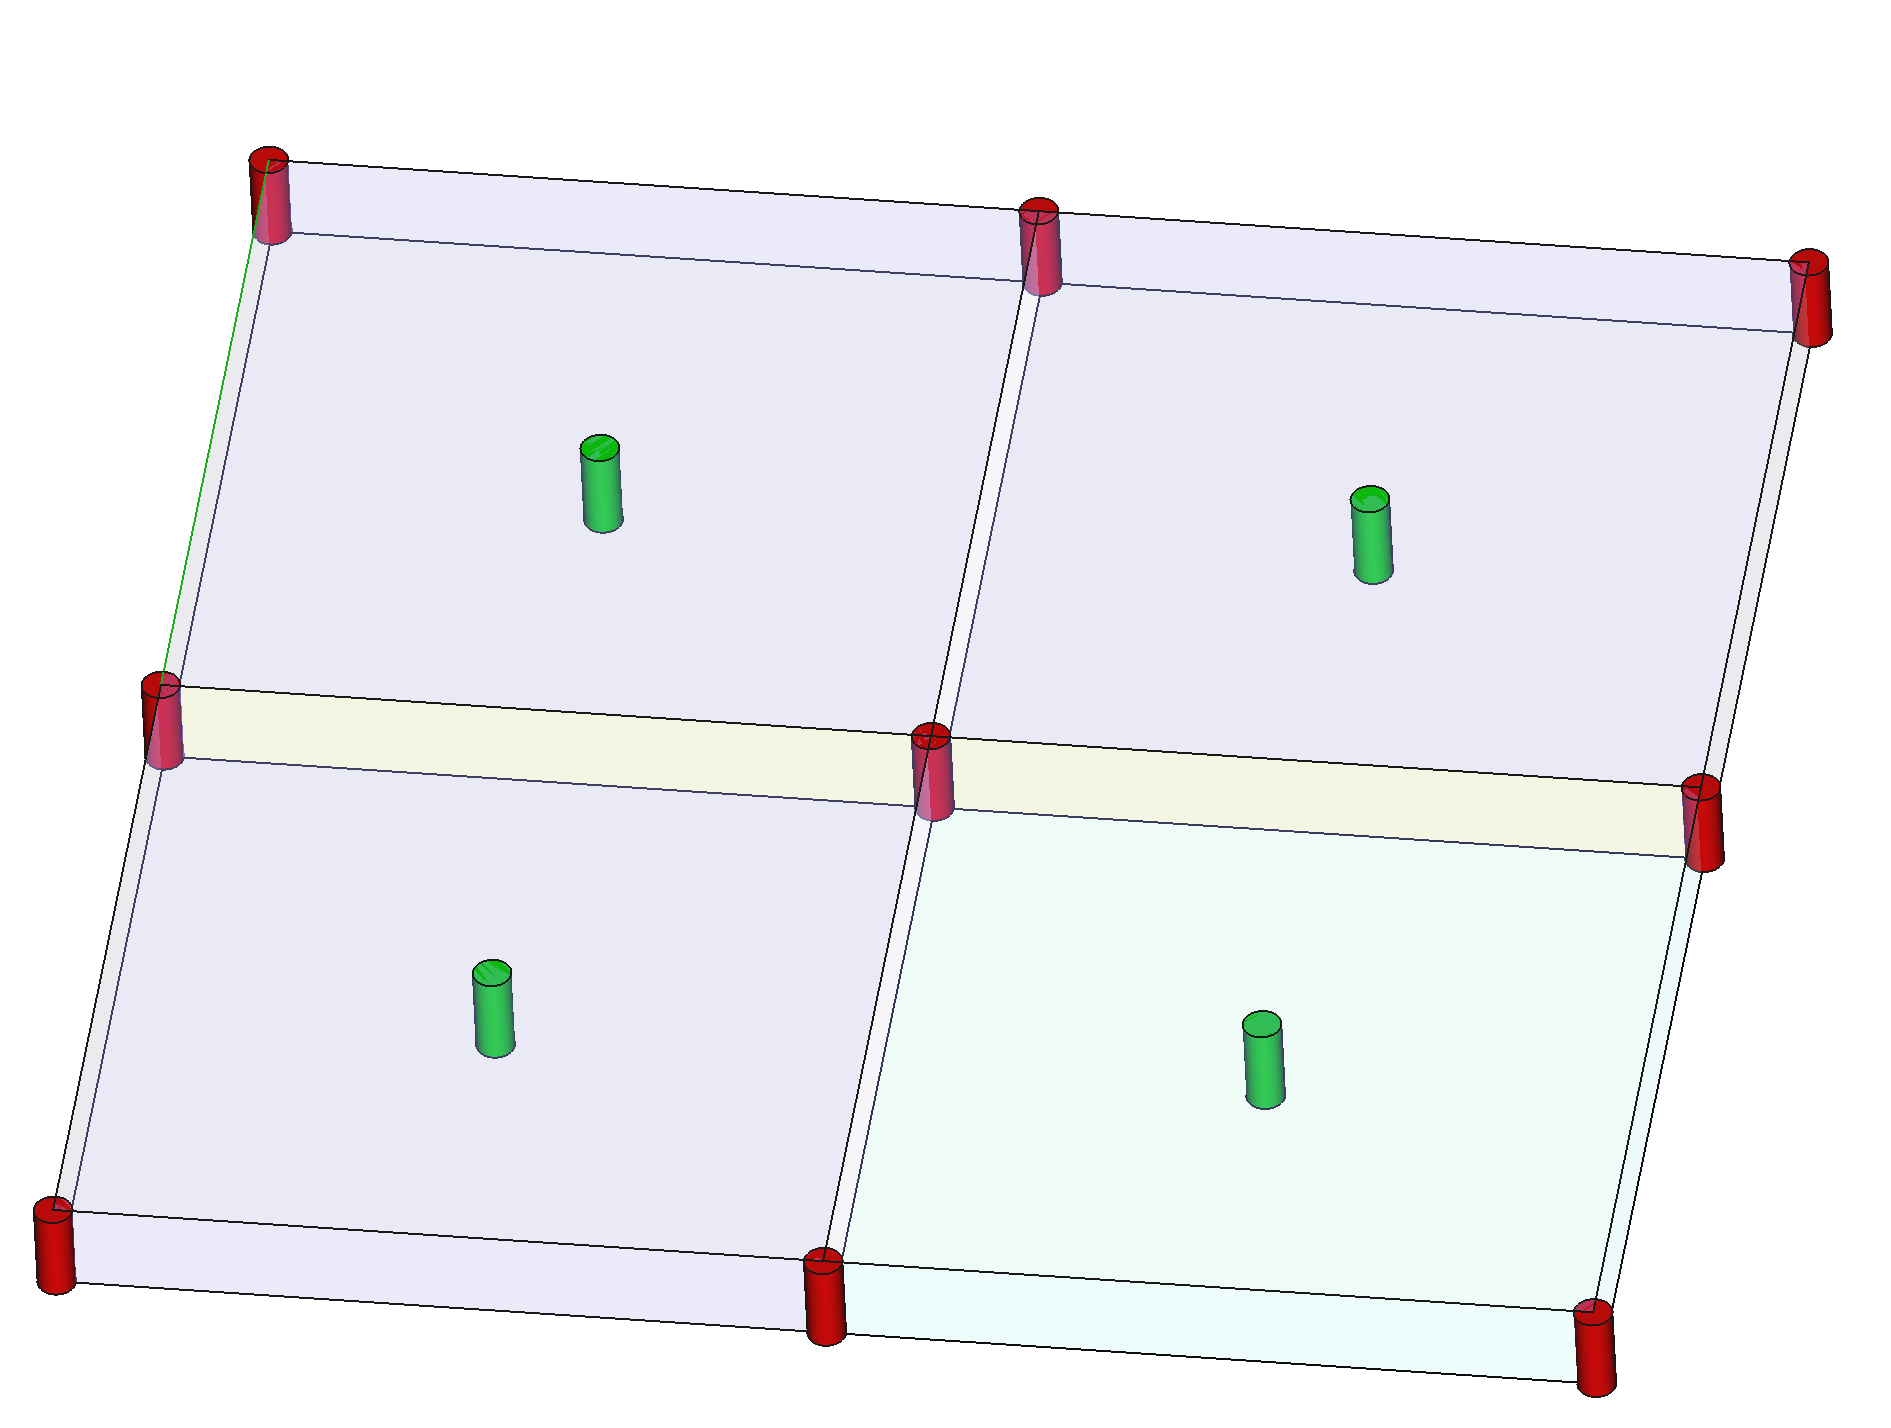
\includegraphics[width=5cm]{3DScheme}
		\caption{array of four 3D cells, bias electrodes in red, readout electrodes in green}
	\end{figure}
\end{frame}

\subsection{3D Diamond Detector}
\begin{frame}
  \frametitle{3D Diamond Detector}
  \begin{itemize}
    \item electrodes formed with a pulsed femto second laser (100 fs pulse; 800 nm wavelength)
    \begin{itemize}
      \item transition of diamond to conducting material (graphitic material i.a.)
    \end{itemize}
    \item different geometries (4 or 6 bias columns)
  \end{itemize}

\end{frame}

% ============================ new frame ==========================================>
\subsection{Beam Tests at CERN}
\begin{frame}
	\frametitle{Beam Tests at CERN}
	\begin{itemize}
		\setlength{\itemsep}{\fill}
		\item using more than 20 years old fixed telescope at SPS at CERN (high spatial resolution)
		\item testing multiple 3D strip detectors
		\item basic working principle has been proven
		\item full charge collection not yet reached in pCVD
		\item improve fabrication technique
	\end{itemize}
	\begin{figure}
		\centering
		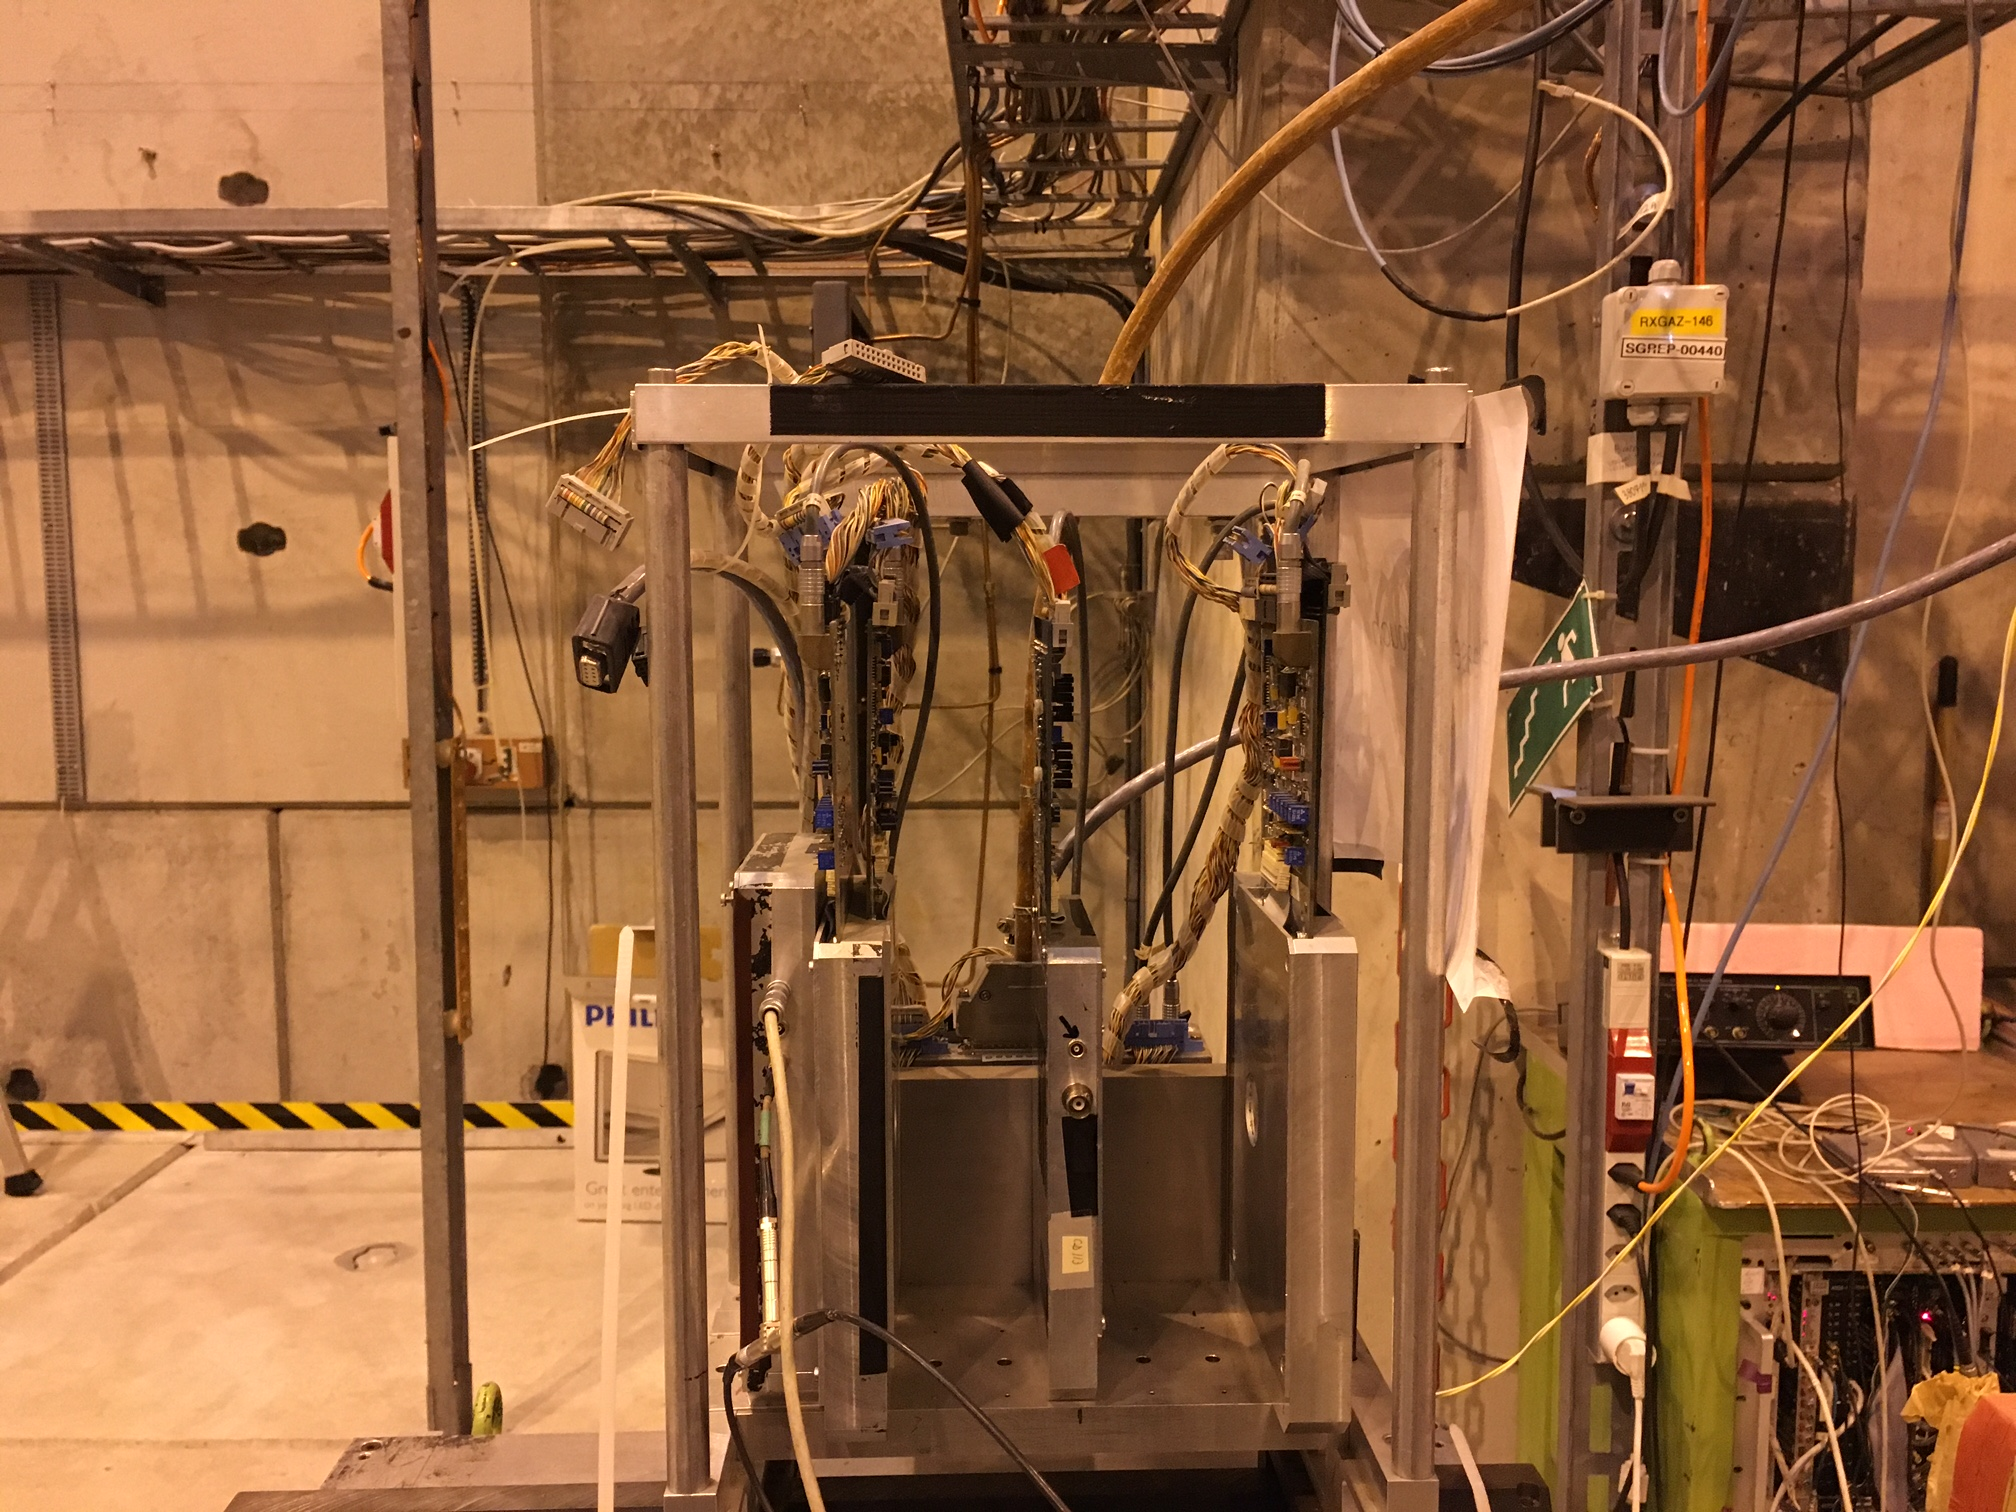
\includegraphics[width=4.5cm]{3DTelescope}
		\caption{Strassbourg Telescope}
	\end{figure}
\end{frame}